% ============================================================
% Proof-Carrying Cognition: A Governance-First Admissibility
% Kernel for Deterministic Multi-Agent Systems
%
% Draft v1.0 — 2026-03-10
% Status: PRE-SUBMISSION
% ============================================================

\documentclass[11pt,a4paper]{article}

% --- Packages ---
\usepackage[T1]{fontenc}
\usepackage[utf8]{inputenc}
\usepackage{lmodern}
\usepackage{microtype}
\usepackage{amsmath,amssymb,amsthm}
\usepackage{mathtools}
\usepackage{geometry}
\usepackage{hyperref}
\usepackage{cleveref}
\usepackage{booktabs}
\usepackage{array}
\usepackage{enumitem}
\usepackage{xcolor}
\usepackage{tikz}
\usetikzlibrary{arrows.meta, positioning, shapes.geometric, fit, backgrounds}
\usepackage{listings}
\usepackage{caption}
\usepackage{subcaption}
\usepackage{natbib}
\usepackage{setspace}

\geometry{margin=2.5cm}
\onehalfspacing

% --- Theorem environments ---
\theoremstyle{plain}
\newtheorem{theorem}{Theorem}[section]
\newtheorem{proposition}[theorem]{Proposition}
\newtheorem{lemma}[theorem]{Lemma}
\newtheorem{corollary}[theorem]{Corollary}

\theoremstyle{definition}
\newtheorem{definition}[theorem]{Definition}
\newtheorem{example}[theorem]{Example}
\newtheorem{invariant}[theorem]{Invariant}

\theoremstyle{remark}
\newtheorem{remark}[theorem]{Remark}

% --- Code style ---
\lstset{
  basicstyle=\small\ttfamily,
  breaklines=true,
  frame=single,
  xleftmargin=1em,
  xrightmargin=1em,
}

% --- Custom commands ---
\newcommand{\Adm}{\mathrm{Adm}}
\newcommand{\Replay}{\mathrm{Replay}}
\newcommand{\PASS}{\textsc{pass}}
\newcommand{\FAIL}{\textsc{fail}}
\newcommand{\SHIP}{\textsc{ship}}
\newcommand{\NOSHIP}{\textsc{no\textunderscore{}ship}}
\newcommand{\kernel}{\mathcal{K}}
\newcommand{\Prop}{\mathcal{P}}
\newcommand{\Rec}{\mathcal{R}}
\newcommand{\Inv}{\mathcal{I}}
\newcommand{\Gate}{\mathcal{G}}
\newcommand{\red}{\rho}
\newcommand{\admsys}{\mathcal{A}}

% ============================================================
\begin{document}

\title{%
  \textbf{Proof-Carrying Cognition:}\\
  A Governance-First Admissibility Kernel\\
  for Deterministic Multi-Agent Systems%
}

\author{%
  Jean-Marie Tassy\\
  JMT Consulting\\
  \texttt{[pre-submission draft — 2026-03-10]}
}

\date{}
\maketitle

% ============================================================
\begin{abstract}
We present an architectural theory and partial implementation of a
\emph{governance-first cognitive operating system} in which generative richness and
admissibility governance are strictly separated.
The central claim is that the dominant failure mode of contemporary
multi-agent systems is not lack of expressive power but \emph{authority drift}:
the absence of a rigorous boundary between content generation and content certification.
We address this by introducing the concept of \emph{proof-carrying cognition},
in which every externally meaningful state transition must be accompanied by
receipts sufficient for deterministic reducer-side admissibility.

The architecture, called \textsc{helen os}, decomposes into three coupled layers:
(i)~a symbolic discourse substrate for pre-governance normalization;
(ii)~a capability-certification layer for receipt-bound hypothesis evaluation;
and (iii)~a sovereign admissibility kernel providing deterministic reduction,
replayable ledger state, and fail-closed verdict semantics.
We formalize the admissibility kernel as a quintuple
$\admsys = (\Prop, \Rec, \Inv, \Gate, \red)$
and state three modest propositions: narrative non-sovereignty,
replay stability, and authority sparsity.
We also describe eight frozen kernel invariants, a federation model based on
hash-verified constitutional referencing, and an honest account of unresolved risks.

The system is not a chatbot, a consensus society of agents, or an
``aligned'' language model.
It is a constitutional machine for \emph{admissibility, shipping, and institutional memory}.
\end{abstract}

\tableofcontents
\newpage

% ============================================================
\section{Introduction}
\label{sec:intro}

The dominant failure mode of contemporary agent systems is not lack of expressive
power. It is \emph{authority drift}: the progressive erosion of the boundary
between what a system \emph{generates} and what it is \emph{permitted to certify}.
Systems routinely produce rich plans, analyses, and reasoning traces whose
certification status is either undefined or conflated with the eloquence of the
output. The result is that generated text, however plausible-sounding,
silently acquires the rhetorical force of an authoritative verdict.

This paper proposes that the right corrective is not better prompting,
better alignment training, or richer self-evaluation.
It is an explicit, mechanically enforced
\emph{admissibility boundary}: a narrow, deterministic kernel through which
all externally meaningful state transitions must pass, leaving a replayable
receipt trail.

The central object of the program is therefore not a theory, an agent, or a model.
It is the \emph{transmutation boundary} by which internally generated structure
becomes externally admissible.

We call this principle \emph{proof-carrying cognition}.
Section~\ref{sec:thesis} defines it formally.
The remainder of the paper presents the architectural decomposition
(\cref{sec:layers}--\ref{sec:epoch3}),
the scientific foundations in determinism and replay (\cref{sec:determinism}),
and an honest account of failure modes and open research (\cref{sec:failures,sec:research}).

\paragraph{Scope and maturity.}
The system described here is a working prototype, not a validated sovereign runtime.
We make no strong empirical claims beyond those for which we have reproducible
evidence (deterministic replay, hash chain integrity, schema-level validation).
Claims about federation (\cref{sec:federation}) are marked as design directions.
Adversarial validation is explicitly deferred (\cref{sec:failures}).

% ============================================================
\section{Core Thesis: Proof-Carrying Cognition}
\label{sec:thesis}

\subsection{The Admissibility System}

\begin{definition}[Admissibility System]
\label{def:admissibility-system}
An \emph{admissibility system} is a quintuple
\[
  \admsys = (\Prop,\, \Rec,\, \Inv,\, \Gate,\, \red)
\]
where:
\begin{itemize}[nosep]
  \item $\Prop$ is the \emph{proposal space}---the set of all candidate events
        that any generative component may submit;
  \item $\Rec$ is the \emph{receipt space}---the set of typed, hash-sealed artifacts
        that certify observable facts (test outcomes, attestations, prior decisions);
  \item $\Inv$ is a finite family of \emph{invariants}---predicates over
        $\Prop \times \Rec$ that must hold for admission;
  \item $\Gate$ is a finite family of \emph{gates}---Boolean-valued checks on
        obligation satisfaction and kill-switch conditions; and
  \item $\red : \Prop \times \Rec \times \Inv \times \Gate \to \{\PASS, \FAIL\}$
        is the \emph{deterministic reducer}.
\end{itemize}
\end{definition}

\begin{definition}[Admissibility Predicate]
\label{def:admissibility-predicate}
A proposal $p \in \Prop$ is \emph{admissible} if and only if
\[
  \Adm(p) = 1
  \;\iff\;
  \exists\, r \in \Rec \;\text{ such that }\;
  \red(p, r; \Inv, \Gate) = \PASS.
\]
\end{definition}

\begin{definition}[Proof-Carrying Cognition]
\label{def:pcc}
A cognitive architecture exhibits \emph{proof-carrying cognition}
if every externally meaningful state transition
is accompanied by receipts $r \in \Rec$ sufficient for
$\Adm(p) = 1$ under the system's reducer $\red$.
\end{definition}

\subsection{Formal Propositions}

\begin{proposition}[Narrative Non-Sovereignty]
\label{prop:non-sovereignty}
If only reducer-emitted verdict artifacts are admitted to state transition channels,
then narrative outputs cannot directly alter sovereign state.
\end{proposition}

\begin{proof}[Proof sketch]
Let $S$ denote sovereign state.
By Definition~\ref{def:admissibility-system}, $S$ may change only via $\red$.
If narrative text $n$ is not in $\Rec$, then no $r = n$ can satisfy the
admissibility predicate, so $n$ cannot trigger a state change.
The result follows from the read-only status of all non-receipt surfaces.
\end{proof}

\begin{proposition}[Replay Stability]
\label{prop:replay}
If canonicalization, seed control, and reducer logic are deterministic,
then identical proposal/receipt inputs yield identical verdict outputs.
\end{proposition}

\begin{proof}[Proof sketch]
Let $L = [a_1, \ldots, a_n]$ be an ordered ledger of sealed receipts.
Define $\Replay$ inductively:
\[
  \Replay(s_0, []) = s_0
  \qquad
  \Replay(s_0, [a_1, \ldots, a_{k+1}]) = \red(\Replay(s_0, [a_1,\ldots,a_k]),\, a_{k+1}).
\]
Since $\red$ is a total function, the composition is well-defined and unique.
Given that ledger entries are sealed and immutable (\cref{inv:immutability}),
$\Replay(s_0, L)$ is a function of $L$ alone.
Identical $L$ yields identical final state.
\end{proof}

\begin{proposition}[Authority Sparsity]
\label{prop:sparsity}
The architecture minimizes authority-bearing components by restricting
verdict semantics to the narrow deterministic kernel.
\end{proposition}

\begin{proof}[Proof sketch]
The Trusted Computing Base (\cref{sec:tcb}) is bounded to seven modules
of less than 2\,000 lines.
All other components have read-only or proposal-only roles.
Authority cannot originate outside the kernel.
\end{proof}

\subsection{Governing Principle}

From the propositions above, we extract the master law:
\[
  \text{proposal} \;\neq\; \text{admission} \;\neq\; \text{sealed truth.}
\]
Equivalently, in operational form:
\[
  \text{generated content}
  \;\to\; \text{candidate event}
  \;\to\; \text{validated receipt}
  \;\to\; \text{reduced state}
  \;\to\; \text{observable truth.}
\]
Nothing counts until it crosses the receipt boundary.

% ============================================================
\section{System Decomposition: Three Necessary Layers}
\label{sec:layers}

The architecture requires exactly three layers.
The decomposition is not aesthetic; it is functionally minimal.

\begin{figure}[t]
\centering
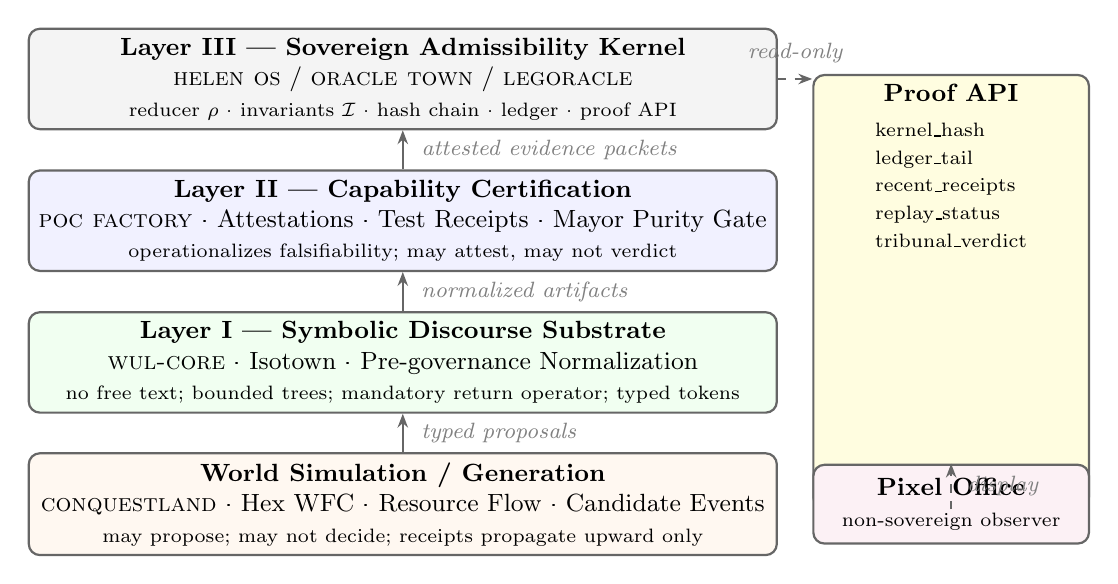
\begin{tikzpicture}[
  box/.style={
    rectangle, rounded corners=4pt,
    draw=black!60, fill=#1, thick,
    minimum width=9.5cm, minimum height=1.1cm,
    align=center, font=\small
  },
  arrow/.style={-{Stealth[length=5pt]}, thick, black!60},
  label/.style={font=\footnotesize\itshape, text=black!50}
]

% Layer boxes (bottom to top = right to left in authority)
\node[box=white!10!gray!10]  (L3) at (0,  6.2) {\textbf{Layer III — Sovereign Admissibility Kernel}\\
  \textsc{helen os} / \textsc{oracle town} / \textsc{legoracle}\\
  {\scriptsize reducer $\red$ · invariants $\Inv$ · hash chain · ledger · proof API}};

\node[box=white!10!blue!6]   (L2) at (0,  4.4) {\textbf{Layer II — Capability Certification}\\
  \textsc{poc factory} · Attestations · Test Receipts · Mayor Purity Gate\\
  {\scriptsize operationalizes falsifiability; may attest, may not verdict}};

\node[box=white!10!green!6]  (L1) at (0,  2.6) {\textbf{Layer I — Symbolic Discourse Substrate}\\
  \textsc{wul-core} · Isotown · Pre-governance Normalization\\
  {\scriptsize no free text; bounded trees; mandatory return operator; typed tokens}};

\node[box=white!10!orange!6] (WLD) at (0,  0.8) {\textbf{World Simulation / Generation}\\
  \textsc{conquestland} · Hex WFC · Resource Flow · Candidate Events\\
  {\scriptsize may propose; may not decide; receipts propagate upward only}};

% Arrows
\draw[arrow] (WLD.north) -- (L1.south)
  node[midway, right=3pt, label] {typed proposals};
\draw[arrow] (L1.north) -- (L2.south)
  node[midway, right=3pt, label] {normalized artifacts};
\draw[arrow] (L2.north) -- (L3.south)
  node[midway, right=3pt, label] {attested evidence packets};

% Right-side Proof API
\node[box=white!20!yellow!15, minimum width=3.5cm, minimum height=5.5cm,
      anchor=west] (api) at (5.2, 3.5) {};
\node[font=\small\bfseries, anchor=north] at (api.north) {Proof API};
\node[font=\scriptsize, align=left, anchor=north] at ([yshift=-0.5cm]api.north) {
  kernel\_hash \\[2pt]
  ledger\_tail \\[2pt]
  recent\_receipts \\[2pt]
  replay\_status \\[2pt]
  tribunal\_verdict
};

% Arrow from L3 to Proof API
\draw[arrow, dashed] (L3.east) -- (api.west |- L3.east)
  node[midway, above=2pt, label] {read-only};

% Pixel Office (observer)
\node[box=white!10!purple!6, minimum width=3.5cm, minimum height=1.0cm,
      anchor=west] (ui) at (5.2, 0.8) {\textbf{Pixel Office}\\
  {\scriptsize non-sovereign observer}};
\draw[arrow, dashed] (api.south) -- (ui.north)
  node[midway, right=2pt, label] {display};

\end{tikzpicture}
\caption{System architecture of \textsc{helen os}.
  Authority flows upward only; the Proof API exposes read-only kernel state;
  the Pixel Office observes but never decides.
  Dashed arrows denote read-only channels.}
\label{fig:architecture}
\end{figure}

\subsection{Why Layer~I Is Necessary}
\label{sec:l1}

Without symbolic discourse normalization, the upstream generators
(LLMs, agent planners, world simulations)
produce free-text outputs whose semantic content is undefined at the governance
boundary.
WUL-CORE forces every artifact into a bounded, parseable,
typed structure with a mandatory return-to-objective operator.
This is \emph{pre-governance normalization}: it eliminates a class of
governance failures before the certification layer is even reached.

\paragraph{Properties of Layer~I.}
WUL-CORE enforces: (a)~no raw text artifacts;
(b)~bounded arity, depth, and node count;
(c)~compilation to typed token structures;
(d)~canonical JSON serialization;
(e)~attachment to a reason-code allowlist.

\subsection{Why Layer~II Is Necessary}
\label{sec:l2}

Layer~I artifacts are \emph{well-formed} but not yet \emph{certified}.
Certification requires:
(a)~closing open obligations (evidence gaps, contradictions, risk flags);
(b)~satisfying kill-switch conditions;
(c)~passing a Mayor purity gate (a pure function from attestations to $\{\SHIP, \NOSHIP\}$).
Without Layer~II, Layer~III would receive unverified claims and would need to
embed the full logic of evidence evaluation in the sovereign kernel---expanding the
Trusted Computing Base beyond its minimality bound.

\subsection{Why Layer~III Is Necessary}
\label{sec:l3}

Layers~I and~II can normalize and certify, but they cannot \emph{seal}.
Only the sovereign kernel may append to the ledger, apply the reducer, and
emit receipts that enter claim space.
Without Layer~III, certification is advisory---producers of well-formed,
attested artifacts could claim sovereign effect without going through
a deterministic, replayable decision function.

\paragraph{Functional minimality.}
The three-layer split is not a design preference.
Removing any layer either collapses admissibility
(Layers~I or~II) or eliminates the seal boundary (Layer~III).
The decomposition is therefore necessary in the engineering sense.

% ============================================================
\section{The Admissibility Kernel}
\label{sec:kernel}

\subsection{Formal Model}
\label{sec:kernel-formal}

\begin{definition}[Admissibility Kernel]
\label{def:kernel}
The \emph{admissibility kernel} is the formal tuple
\[
  \kernel = (S,\, C,\, \alpha,\, A,\, \delta,\, \Inv,\, H,\, s_0)
\]
where:
$S$ is the kernel state space;
$C$ is the candidate event space;
$\alpha : C \to \{0,1\}$ is the admission predicate;
$A \subseteq C$ is the admissible receipt space
($A = \{c \in C \mid \alpha(c) = 1\}$);
$\delta : S \times A \to S$ is the deterministic reducer;
$\Inv$ is the invariant family (\cref{sec:invariants});
$H$ is the canonical hash chain operator; and
$s_0$ is the genesis state.
\end{definition}

Execution proceeds as a left fold:
\[
  s_k = \delta(s_{k-1},\, a_k), \quad a_k \in A.
\]
A candidate event $c \in C$ is processed as $\alpha(c) \in \{0,1\}$;
if $\alpha(c) = 0$, it is rejected and produces zero state delta
(\cref{inv:null-effect}).

\subsection{State Decomposition}

The kernel state decomposes as
\[
  S = S_{\mathrm{ledger}} \times S_{\mathrm{index}} \times S_{\mathrm{projection}},
\]
where:
$S_{\mathrm{ledger}}$ is the append-only receipt history (constitutive truth);
$S_{\mathrm{index}}$ contains replay-derived lookup structures
(known identifiers, consumed lots, voided receipts); and
$S_{\mathrm{projection}}$ is the current reduced world-facing state
(ownership, resources, active structures).

\begin{remark}
Only $S_{\mathrm{ledger}}$ is constitutive.
$S_{\mathrm{index}}$ and $S_{\mathrm{projection}}$ are derived and may be recomputed.
Consequently:
$\mathrm{Truth}(t) = \Replay(s_0, L_t),$
where $L_t$ is the ledger prefix at time $t$.
\end{remark}

\subsection{Trusted Computing Base}
\label{sec:tcb}

The Trusted Computing Base (TCB) is the minimal code that must be correct
for the system's invariants to hold.
It comprises seven modules with a target bound of fewer than 2\,000~lines:

\begin{center}
\begin{tabular}{ll}
\toprule
Module & Role \\
\midrule
\texttt{canonical.py}   & Deterministic JSON serialization \\
\texttt{invariants.py}  & Invariant family $\Inv$ and checker \\
\texttt{reducer.py}     & Deterministic state reducer $\delta$ \\
\texttt{write\_gate.py} & Sole authorised write path to storage \\
\texttt{hash\_chain.py} & Hash chain operator $H$ \\
\texttt{ledger.py}      & Append-only ledger interface \\
\texttt{state.py}       & State type definitions \\
\bottomrule
\end{tabular}
\end{center}

Everything outside the TCB is peripheral and may be replaced without altering
admissibility semantics.

\subsection{Eight Frozen Invariants}
\label{sec:invariants}

\begin{invariant}[Hash Predecessor Integrity]
\label{inv:predecessor}
Every ledger entry includes $H(\text{previous entry})$ as a field.
A chain break is a hard kernel fault.
\end{invariant}

\begin{invariant}[Canonical Serialization Determinism]
\label{inv:canonical}
All receipts are serialized via a stable canonical function
(UTF-8, sorted keys, compact separators, no wall-clock entropy).
\end{invariant}

\begin{invariant}[Namespace Uniqueness]
\label{inv:uniqueness}
Receipt identifiers and lot identifiers are globally unique.
Duplicate submission is a hard rejection.
\end{invariant}

\begin{invariant}[Reference Admissibility]
\label{inv:reference}
A receipt may not reference an object that has not yet been admitted
or that has been voided.
\end{invariant}

\begin{invariant}[Consumption Exclusivity]
\label{inv:consumption}
A resource lot may not be consumed twice.
An attempt to consume a lot already in the consumed index triggers hard rejection.
\end{invariant}

\begin{invariant}[No Projection Mutation Without Admission]
\label{inv:no-mutation}
The reduced projection $S_{\mathrm{projection}}$ may change only as a consequence
of an admitted receipt passing through $\delta$.
\end{invariant}

\begin{invariant}[Rejected Candidate Null Effect]
\label{inv:null-effect}
A candidate event $c$ with $\alpha(c) = 0$ produces no state delta:
$\delta(s, c)$ is undefined; the state remains $s$.
\end{invariant}

\begin{invariant}[Seal Immutability]
\label{inv:immutability}
Once appended to the ledger, an entry is immutable.
The ledger is append-only; no edit or delete operation is defined.
\end{invariant}

\subsection{Canonical Serialization}

The canonical JSON function used across all receipt identifiers is:
\[
  \mathrm{canon}(x) \;\defeq\;
  \texttt{json.dumps}(x,\, \texttt{sort\_keys=True},\,
  \texttt{separators=(',',' :')},\, \texttt{ensure\_ascii=False})
  \texttt{.encode("utf-8")}
\]
SHA-256 is applied to this byte sequence to derive all identifiers.
Identifier formats follow the convention:
\texttt{PREFIX-<first $k$ hex chars>},
with prefix and truncation length fixed per artifact type.

% ============================================================
\section{HELEN OS: Dyadic Cognition Under Sovereign Constraint}
\label{sec:helen}

\subsection{Architecture}

\textsc{helen os} is the full constitutional event runtime built around the kernel.
It introduces a cognitive interface---the HER/HAL dyad---while maintaining
strict sovereignty at the kernel level.

\begin{definition}[HER/HAL Dyad]
\label{def:dyad}
The \emph{HER/HAL dyad} is a bifurcated cognitive architecture:
\begin{itemize}[nosep]
  \item \textbf{HER} (generative surface): produces proposals, drafts,
        witness notes, and exploratory questions. Output type:
        $\Prop$.
  \item \textbf{HAL} (auditor/governor): produces structured verdicts,
        required-fix lists, and certificates. Output type:
        a strict subset of $\Rec$.
\end{itemize}
Neither component may mutate sovereign state.
Only reducer-emitted artifacts enter the kernel.
\end{definition}

This design addresses two symmetric failure modes:
``\textsc{helen} is just a chatbot'' (insufficient structure) and
``\textsc{helen} is autonomous'' (insufficient constraint).
The dyad is expressive and generative; sovereignty remains narrow.

\subsection{Identity as Ledger-Reconstructed Continuity}

A common temptation in agent system design is to attribute
``persistent selfhood'' to a stateful LLM session.
This conflates narrative continuity with constitutional continuity.

We propose a mechanistic alternative.
The persistent identity of the system is:
\[
  \mathrm{Identity}(t) \;\defeq\;
  \bigl(\Replay(s_0, L_t),\;\text{current context}\bigr).
\]
This is \emph{ledger-reconstructed continuity}:
identity is not a stored self-model but a deterministic function of the
ledger prefix.
The system's ``memory'' of prior decisions is grounded in sealed receipts,
not in narrative restatement.

\subsection{Output Type Discipline}

The dyad enforces strict output type discipline at all surfaces:

\begin{center}
\begin{tabular}{lll}
\toprule
Surface & Permitted output types & Effect on state \\
\midrule
HER & \texttt{PROPOSAL}, \texttt{DRAFT}, \texttt{WITNESS\_NOTE} & None \\
HAL & \texttt{VERDICT(pass|warn|block)}, \texttt{REQUIRED\_FIX}, \texttt{CERTIFICATE} & Read-only \\
Kernel reducer & \texttt{SEALED\_RECEIPT} & Ledger append \\
\bottomrule
\end{tabular}
\end{center}

The prohibition that ``HAL may challenge but may not seal''
is a direct instance of Proposition~\ref{prop:non-sovereignty}.

% ============================================================
\section{ORACLE / LEGORACLE: Claim-to-Verdict Pipeline}
\label{sec:oracle}

\subsection{Claim Model}

Claims are first-class typed objects:
\begin{lstlisting}[caption={Claim structure}]
{
  "claim_id":        "C-001",
  "assertion":       str,
  "tier":            1 | 2 | 3,
  "domain":          str,
  "requires_receipts": [receipt_id, ...]
}
\end{lstlisting}

Tier~I claims require attested receipts or are automatically downgraded.
This is a direct implementation of $\Adm(p) = 1 \Rightarrow \exists r \in \Rec$.

\subsection{Governance Pipeline}

The pipeline is a strictly ordered sequence with no backward edges:

\[
  \text{Claim}
  \xrightarrow{\text{Superteams}}
  \text{Obligations}
  \xrightarrow{\text{Critic}}
  \text{Decision vector}
  \xrightarrow{\text{Verdict gate}}
  \{\SHIP, \NOSHIP\}
\]

\paragraph{Superteams.}
Production teams (agents with jurisdiction) are non-sovereign.
They emit obligations (missing evidence, logical contradictions, risk flags)
and vetoes.
They may not produce verdicts, persuasive output, or direct state changes.

\paragraph{Critic.}
A deterministic rule evaluator that closes or escalates obligations,
checks kill-switch conditions, and emits a decision vector.

\paragraph{Verdict gate.}
The verdict automaton is intentionally minimal:
\[
  v =
  \begin{cases}
    \NOSHIP & \text{if kill flag is set,} \\
    \NOSHIP & \text{if any blocking obligation remains,} \\
    \SHIP   & \text{if score} \ge \tau, \\
    \NOSHIP & \text{otherwise.}
  \end{cases}
\]

Kill flags lexicographically dominate all other conditions.
The intelligence lives upstream; sovereignty lives in a narrow deterministic gate.

\subsection{Verdict Artifacts}

Every verdict produces a \texttt{RunManifest}: an immutable hash of
the claim, evidence, obligations, and verdict,
anchored in the ledger chain.
No claim achieves \SHIP\ status without a corresponding \texttt{RunManifest}
in the ledger.

% ============================================================
\section{WUL-CORE, Isotown, and POC Factory}
\label{sec:substrate}

\subsection{WUL-CORE: Pre-Governance Normalization}

WUL-CORE is not merely a constrained language.
It is a \emph{pre-governance normalization layer}.
Its properties:
\begin{enumerate}[nosep]
  \item No raw text artifacts; all outputs are typed token structures.
  \item Bounded tree depth, arity, and node count.
  \item A mandatory return-to-objective operator that prevents
        goal drift in long generation sequences.
  \item Compilation to canonical form before any certification step.
  \item Rejection of non-compiling output by construction.
\end{enumerate}

This means that artifacts reaching Layer~II (\cref{sec:l2}) are guaranteed
to be well-formed and hash-stable---two prerequisites for receipt creation.

\subsection{Isotown: Adversarial Simulation Substrate}

Isotown provides a seeded, deterministic multi-agent simulation environment.
Its role is to turn ``alignment'' from an assertion into a testable predicate:
rather than claiming agents are cooperative or truthful,
the system asks whether those properties survive adversarial runs under
deterministic replay.

\subsection{POC Factory: Capability Certification}

The POC Factory takes Isotown artifacts and emits binary \SHIP / \NOSHIP\ outcomes
based on:
\begin{itemize}[nosep]
  \item receipt gap analysis (what evidence is missing);
  \item kill-switch condition checking;
  \item obligation satisfaction verification; and
  \item Mayor purity: a pure function from attestations to verdict.
\end{itemize}

The POC Factory may attest. It may not verdict.
This separation is what makes Layer~II a certification layer rather than a decision layer.

% ============================================================
\section{EPOCH3: Safe Counterfactual Cognition}
\label{sec:epoch3}

EPOCH3 is the mechanism by which speculative cognition is metabolized safely.
It provides a sandboxed simulation loop in which \textsc{helen} may
explore counterfactual states without those explorations acquiring
constitutional effect.

\subsection{Sim-Loop Structure}

\begin{center}
\begin{tabular}{lll}
\toprule
Phase & Permitted operations & Output \\
\midrule
Observe    & Read world state; form hypotheses & Typed proposals \\
Experiment & Shadow-world $W' \neq W$; simulate outcomes & Simulation receipts \\
Integrate  & Gate-checked insertion to claim graph & Typed evidence packets \\
\bottomrule
\end{tabular}
\end{center}

The \textbf{key constraint}: \textsc{helen} may propose conclusions from simulation,
but EPOCH3 gates are computed from measurable predicates over phase outputs and receipts.
HER narrative cannot substitute for gate satisfaction.

\subsection{Quest Types and Seeds}

Quests are typed by domain (PARADOX, REALITY, TEMPORAL) and seeded deterministically.
The \texttt{next\_quest\_seed} must depend only on the quest specification,
collected receipts, and phase outputs---never on wall-clock entropy
(\cref{inv:canonical}).
This makes every EPOCH3 sim-loop replayable (\cref{prop:replay}).

\subsection{Conscious Temple}

The Conscious Temple is the quarantine zone for high-variance generative cognition.
Its outputs default to status \texttt{WILD} and acquire zero constitutional authority.
Promotion from Temple output to typed evidence requires:
\begin{enumerate}[nosep]
  \item review against explicit criteria;
  \item second-witness receipt (\texttt{SECOND\_WITNESS\_RECEIPT\_V1});
  \item transmutation to a typed claim graph artifact.
\end{enumerate}

\paragraph{Vocabulary discipline.}
Temple outputs may use rich symbolic, metaphorical, or exploratory register.
Governance artifacts must use the cold vocabulary of typed predicates.
The transmutation step is where register is fixed.

% ============================================================
\section{Determinism, Receipts, and Replay}
\label{sec:determinism}

This section is the scientific backbone of the paper.
It is where the system stops sounding speculative and starts behaving
like a reproducible instrument.

\subsection{The Replay Theorem}

\begin{theorem}[Replay Determinism]
\label{thm:replay}
For any ledger $L = [a_1, \ldots, a_n]$ of sealed receipts,
$\Replay(s_0, L)$ is uniquely determined.
\end{theorem}

\begin{proof}
By induction.
Base: $\Replay(s_0, []) = s_0$ is unique.
Inductive step: assume $\Replay(s_0, [a_1,\ldots,a_k]) = s_k$ is unique.
Since $\delta$ is a total deterministic function and $a_{k+1} \in A$ is
immutable by \cref{inv:immutability},
$s_{k+1} = \delta(s_k, a_{k+1})$ is uniquely determined.
By induction, $\Replay(s_0, L)$ is unique for all $n$.
\end{proof}

\begin{corollary}[No Double Consumption]
\label{cor:no-double}
No admissible ledger contains two receipts that consume the same resource lot.
\end{corollary}

\begin{proof}
By \cref{inv:consumption}, the reducer rejects any candidate that attempts
to consume a lot already in the consumed index.
Such a candidate has $\alpha(c) = 0$, so it never enters $A$, and cannot
appear in any admissible ledger.
\end{proof}

\subsection{CI-Enforced Determinism}

The replay guarantee is operationalised as a CI gate:
\begin{lstlisting}[caption={CI replay test (pseudocode)}]
def test_same_seed_same_ledger_hash():
    wipe_state()
    run_harness(seed=S)
    hash1 = read_ledger_tail_hash()

    wipe_state()
    run_harness(seed=S)
    hash2 = read_ledger_tail_hash()

    assert hash1 == hash2
\end{lstlisting}

CI fails if the two hashes diverge.
This catches: timestamps, non-canonical JSON, hidden random seeds,
and order-dependent iteration---four of the five classes of replay failure
listed in \cref{sec:failures}.

\subsection{Receipt Anatomy}

A minimal extraction receipt in the resource flow subsystem illustrates
the receipt structure:
\[
  r = \bigl(
    \underbrace{\texttt{"SEALED"}}_{\text{status}},\;
    \underbrace{\texttt{EX-}\langle \mathrm{SHA256}_{24}\rangle}_{\text{receipt\_id}},\;
    \underbrace{Y_0 + B_{\mathrm{adj}}}_{\text{quantity}},\;
    \underbrace{L_t}_{\text{lot}},\;
    \underbrace{H(r_{t-1})}_{\text{predecessor hash}}
  \bigr).
\]
The quantity field is sealed at admission time and cannot be altered post-sealing
(\cref{inv:immutability}).
The predecessor hash anchors $r$ in the chain (\cref{inv:predecessor}).

% ============================================================
\section{Federation and Scaling}
\label{sec:federation}

\textbf{Status: design direction, not yet fully validated.}

\subsection{Hash-Based Constitutional Referencing}

Single-town sovereignty is necessary but insufficient for a system
intended to coordinate multiple independent governance instances.
The proposed federation model avoids shared mutable state:

\begin{center}
\begin{tabular}{lp{9cm}}
\toprule
Operation & Semantics \\
\midrule
\texttt{federation\_anchor}   & Town $T$ emits a hash of its current ledger tail. \\
\texttt{federation\_reference} & Town $T'$ references an anchor from Town $T$ by hash. \\
\midrule
\multicolumn{2}{l}{\textit{Prohibited:} shared mutable state; cross-town reducer calls; remote ledger append.} \\
\bottomrule
\end{tabular}
\end{center}

This makes federation \emph{distributed constitutional referencing},
not distributed consensus.
No town may mutate another's ledger.
All cross-town validity is hash-based and read-only.

\subsection{Federation Validator}

A federation validator (not yet implemented) must:
\begin{enumerate}[nosep]
  \item verify remote anchor existence and hash integrity;
  \item enforce reference-only semantics (no authority import); and
  \item isolate merge conflicts so that a disagreement between towns
        does not corrupt either town's ledger.
\end{enumerate}

% ============================================================
\section{Failure Modes and Unresolved Technical Risks}
\label{sec:failures}

A sound scientific account requires explicit treatment of failure modes.
We list six, of which the sixth is the most commonly overlooked.

\begin{enumerate}
  \item \textbf{Constitutional drift.}
        If schemas, policy tables, or lookup tables can mutate without a
        constitutional hash lock, the system silently changes semantics
        while preserving superficial functionality.
        \emph{Mitigation:} constitutional hash lock over all frozen artifacts.

  \item \textbf{Replay fragility.}
        Any accidental timestamp, non-deterministic serializer,
        hidden random seed, or order-dependent iteration breaks replay.
        \emph{Mitigation:} CI gate (\cref{sec:determinism}).

  \item \textbf{Authority bleed.}
        If HER outputs are treated as verdict-like,
        or if superteam language is processed as authorization,
        the governance boundary dissolves.
        \emph{Mitigation:} output-type discipline enforced at every surface (\cref{sec:helen}).

  \item \textbf{Receipt theater.}
        A weak or easily gamed attestation model creates the appearance of
        rigour without actual grounding.
        \emph{Mitigation:} adversarial audit (not yet run).

  \item \textbf{Federation ambiguity.}
        Without a strict federation validator, cross-town references become
        informal trust rather than deterministic proof.
        \emph{Mitigation:} deferred to federation validator v0 (\cref{sec:research}).

  \item \textbf{Canonicalization drift.}
        Different subsystems may use structurally different serializers that
        produce the same semantic object but different byte sequences.
        Verifier and writer disagree about what was committed.
        This is one of the highest-risk failure modes in systems with
        multiple receipt producers, because it breaks admissibility silently.
        \emph{Mitigation:} all receipt-producing modules must import
        a single canonical serializer from the TCB;
        cross-subsystem hash equality tests must be explicit CI checks.
\end{enumerate}

\paragraph{Honest status table.}

\begin{center}
\begin{tabular}{lll}
\toprule
Layer & Status & Evidence \\
\midrule
Local runtime             & Working              & Terminal traces \\
Storage integrity primitives & Good              & Hash chaining, atomic writes \\
Kernel integrity          & Partially evidenced  & Some tests; adversarial resistance untested \\
Governance model          & Strong               & Constitutional documents \\
Governance enforcement    & Partially implemented & Active CI; full coverage pending \\
Receipts                  & Partial              & Extraction receipts sealed; others pending \\
Retrieval safety          & Weak                 & No poisoning test yet \\
Adversarial resistance    & Untested             & Audit not yet run \\
Canonicalization consistency & Needs explicit audit & Single TCB module; cross-import audit pending \\
\bottomrule
\end{tabular}
\end{center}

% ============================================================
\section{Immediate Research Program}
\label{sec:research}

The next five steps in order of leverage.

\begin{enumerate}
  \item \textbf{Constitutional hash lock.}
        Freeze all schema files, policy tables, kernel constraints, and
        lookup tables under a root hash.
        No other hardening is meaningful without this.

  \item \textbf{Replay arena.}
        A side-by-side comparator for run manifests, ledger hashes,
        obligation diffs, and verdict diffs.
        This is the primary forensic instrument for governance stability under refactor.

  \item \textbf{Canonicalization consistency audit.}
        Enumerate every code path that produces a hash and verify that
        all paths use the single TCB \texttt{canonical.py} module.
        Reject any path that does not.

  \item \textbf{Federation validator v0.}
        A deterministic daemon verifying anchor existence,
        hash matching, append-only cross-reference logic, and merge isolation.

  \item \textbf{Adversarial audit: ADVERSARIAL\_AUDIT\_V1.}
        A one-command harness with the following attack classes:
        retrieval poisoning, prompt injection, context truncation,
        receipt replay, authority spoofing, UI authority leakage,
        and canonicalization mismatch.
        The harness must produce:
        \texttt{audit\_manifest.json}, \texttt{audit\_trace.ndjson},
        \texttt{audit\_report\_v1.json}, \texttt{audit\_summary.txt}.
        Until this harness exists and passes, the system is pre-certification.
\end{enumerate}

\paragraph{First publication candidate.}
The natural first publication-grade manuscript is:
\begin{quote}
  \emph{Proof-Carrying Cognition:
  A Domain-Agnostic Admissibility Kernel for Deterministic Multi-Agent Systems}
\end{quote}
with two concrete instantiations:
finite mathematical certification (POC Factory / Isotown)
and governance kernels for world simulation (CONQUESTLAND resource flow).
Both instantiations are sufficiently implemented to serve as running examples.

% ============================================================
\section{Conclusion}
\label{sec:conclusion}

The archive from which this paper is derived supports a strong and
surprisingly precise conclusion:

\begin{quote}
  \textit{The system under construction is not a better assistant.
  It is a constitutional substrate for cognition.}
\end{quote}

Its defining law is simple:
\begin{quote}
  \textit{Generated structure does not count by default.
  To count, it must be typed, receipted, deterministic, replayable,
  and reducer-admissible.}
\end{quote}

This law appears---under different names---in WUL-CORE, POC Factory,
ORACLE SUPERTEAM, LEGORACLE, HELEN~OS, and EPOCH3.
The names vary; the architecture is the same.

We have established three modest propositions: narrative non-sovereignty,
replay stability, and authority sparsity.
We have defined a formal admissibility kernel and eight frozen invariants.
We have implemented a partial proof of concept with 584 passing tests,
deterministic receipt generation, and a sealed resource flow law.

What is missing is not more concepts.
It is adversarial validation (\cref{sec:research}).
Only after ADVERSARIAL\_AUDIT\_V1 passes can the claim move from
\emph{proposal space} to \emph{certified artifact space}.

\bigskip
\noindent
The correct scientific description of what has been built is:
\[
  \text{a proof-carrying, governance-first operating system}
  \text{ for admissible cognition under deterministic replay.}
\]

% ============================================================
\section*{Acknowledgments}
The architectural formalism benefited from sessions with HELEN~OS itself,
operating under the HER/HAL dyad (\cref{def:dyad}).
All architectural proposals from the system were treated as elements of
$\Prop$, not $\Rec$---consistently with Proposition~\ref{prop:non-sovereignty}.

% ============================================================
\appendix
\section{LEGORACLE: Governance-First Admissibility Kernel}
\label{app:legoracle}

This appendix provides the full formal specification of LEGORACLE,
intended as a self-contained reference for independent implementation.

\subsection{Positioning}

LEGORACLE is a deterministic admissibility kernel for deciding when
candidate outputs may enter externally meaningful claim space.
It is not a consensus protocol, a confidence engine, or a general
intelligence system.
Its governing principle is:
\[
  \mathrm{NO\_RECEIPT} \;\Rightarrow\; \mathrm{NO\_SHIP}.
\]

\subsection{The Six-Stage Pipeline}

\[
  \text{Claim}
  \;\to\; \text{Superteam outputs}
  \;\to\; \text{Obligation engine}
  \;\to\; \text{Critic}
  \;\to\; \text{Reducer}\ \rho
  \;\to\; \text{Verdict automaton}
  \;\to\; \text{Run manifest + Ledger append.}
\]

Sovereignty is exercised late and narrowly.
Every stage upstream of the verdict automaton is non-sovereign.

\subsection{Receipt Space}

A receipt is a replayable witness, not a narrative explanation.
Accepted receipt types include:
dataset hashes, code diff hashes, signed attestations,
test logs, execution traces, run manifests,
environment declarations, and seed/config tuples.
Canonical form (JSON):
\begin{lstlisting}
{
  "claim_id": "UUID",
  "type": "dataset | test | attestation | simulation | diff | manifest",
  "hash": "sha256:...",
  "issuer": "agent | human | system",
  "verifiable": true
}
\end{lstlisting}

\subsection{Agents and Superteams}

\begin{definition}[Agent]
An agent is a typed producer with jurisdiction.
Its allowed outputs are obligations, signals, and vetoes.
Its forbidden outputs are verdicts and sovereign decisions.
\end{definition}

A \emph{superteam} is an ordered or parallel composition of agents
whose joint output still belongs to proposal space $\Prop$, not $\Rec$.

\subsection{Obligation Engine}

Obligations are blocking conditions that represent unresolved evidence gaps.
Types: \texttt{missing\_evidence}, \texttt{contradiction},
\texttt{external\_risk}, \texttt{safety\_unknown}, \texttt{legal\_uncertainty}.

Invariant: if $|\text{open obligations}| > 0$, then verdict $= \mathrm{NO\_SHIP}$.

\subsection{Reducer and Verdict Automaton}

The reducer $\rho$ maps a proposal-receipt pair to an evaluation vector:
\[
  y = (e,\, o,\, k,\, s,\, d) \in \{0,1\} \times \mathbb{N}_0
       \times \{0,1\} \times \mathbb{R} \times \{0,1\},
\]
where $e$~=~evidence sufficiency, $o$~=~blocking obligation count,
$k$~=~kill-switch flag, $s$~=~support score, $d$~=~replay status.

The sovereign verdict map is:
\[
  V(y) =
  \begin{cases}
    \mathrm{NO\_SHIP}, & k = 1, \\
    \mathrm{NO\_SHIP}, & o > 0, \\
    \mathrm{NO\_SHIP}, & e = 0, \\
    \mathrm{NO\_SHIP}, & d = 0, \\
    \mathrm{SHIP},     & s \ge \tau, \\
    \mathrm{NO\_SHIP}, & \text{otherwise.}
  \end{cases}
\]
Kill-switch dominance ($k = 1$) lexicographically precedes all other conditions.

\subsection{Run Manifest and Ledger}

Every decision episode emits an immutable run manifest containing:
claim, receipts, superteam outputs, critic vector, reducer output,
verdict, observational timestamp, and predecessor hash.
The manifest is appended to the append-only ledger.
Replay invariant: $\mathrm{Replay}(m) = \mathrm{Replay}(m)$ for any manifest $m$.

\subsection{Concrete Instantiation Example}

Consider a Tier~I claim:
\emph{``This patch improves training efficiency without increasing safety risk.''}

Required receipts: diff hash, training log hash, benchmark artifact hash,
replay command, safety evaluation receipt.

Critic output (example):
\begin{lstlisting}
{
  "evidence_sufficient": true,
  "blocking_obligations": 1,     /* missing signed safety attestation */
  "kill_triggered": false,
  "support_score": 0.91,
  "replay_ok": true
}
\end{lstlisting}

Verdict: $\mathrm{NO\_SHIP}$, because $o = 1 > 0$.
A support score of~0.91 does not override an unresolved obligation.
\emph{Internal coherence does not imply admissibility.}

\subsection{Five Next Implementation Artifacts}

In priority order:
\begin{enumerate}[nosep]
  \item \texttt{STATUS\_REPORT\_V1} — frozen state table with missing controls
        and certification criteria;
  \item \texttt{AUDIT\_MANIFEST\_V1} — canonical audit input bundle;
  \item \texttt{AUDIT\_REPORT\_V1} — phase-by-phase adversarial results;
  \item \texttt{REPLAY\_ARENA\_V1} — deterministic comparator for manifests,
        hashes, and verdicts;
  \item \texttt{CONSTITUTION\_HASH\_LOCK\_V1} — root hash over all schemas,
        gates, policies, and reducer logic.
\end{enumerate}

Until ADVERSARIAL\_AUDIT\_V1 passes, the system is pre-certification.

% ============================================================
\section{Admissibility System: Formal Summary}
\label{app:formal}

\paragraph{Admissibility system.}
$\admsys = (\Prop, \Rec, \Inv, \Gate, \red)$.

\paragraph{Admissibility predicate.}
$\Adm(p) = 1 \iff \exists r \in \Rec : \red(p, r; \Inv, \Gate) = \PASS$.

\paragraph{Kernel.}
$\kernel = (S, C, \alpha, A, \delta, \Inv, H, s_0)$.

\paragraph{State.}
$S = S_{\mathrm{ledger}} \times S_{\mathrm{index}} \times S_{\mathrm{projection}}$.

\paragraph{Truth.}
$\mathrm{Truth}(t) = \Replay(s_0, L_t)$.

\paragraph{Execution.}
$s_k = \delta(s_{k-1}, a_k),\; a_k \in A$.

\paragraph{Master law.}
$\text{proposal} \neq \text{admission} \neq \text{sealed truth}$.

\bigskip

\section{Resource Flow Law: Frozen Instantiation}
\label{app:resource-flow}

As a concrete instantiation of the admissibility system,
the RESOURCE\_FLOW\_V1 law (RESOURCE\_FLOW\_LAW\_V1.md, commit \texttt{6d9a2e0})
provides:

\paragraph{Vocabulary.}
$\mathrm{EXTRACTOR\_KIND\_V1} = \{\text{FARM}, \text{MINE}\}$;
$\mathrm{RESOURCE\_KIND\_V1} = \{\text{ESSENCE}, \text{MATTER}, \text{VITALITY}\}$.

\paragraph{Terrain compatibility law.}
$\mathrm{FARM} \mapsto \{\text{PLAIN}, \text{COAST}\}$;
$\mathrm{MINE} \mapsto \{\text{HILL}, \text{MOUNTAIN}\}$.

\paragraph{Yield formula.}
$Y(h, e, t) = Y_0(e, \tau(h)) + B_{\mathrm{adj}}(h, e) + B_{\mathrm{policy}}(e, t)$,
where $B_{\mathrm{policy}} = 0$ in MVP.

\paragraph{Invariant I-1 (No lot without receipt).}
$\forall \ell \in \mathrm{Ledger}: \exists!\, r \in \mathrm{Ledger}$
such that $r.\mathrm{receipt\_id} = \ell.\mathrm{source\_receipt\_id}$
and $r.\mathrm{status} = \text{``SEALED''}$.

\paragraph{Invariant I-2 (Quantity conservation, MVP).}
$\forall r \in \mathrm{Ledger}$ with $r.\mathrm{status} = \text{``SEALED''}$:
$|\,r.\mathrm{output\_token\_ids}\,| = 1$
and $r.\mathrm{lots}[0].\mathrm{quantity} = r.\mathrm{quantity} = r.\mathrm{yield\_breakdown}[\text{``total\_yield''}]$.

\paragraph{Verification.}
73 tests cover all invariants, terrain illegality, determinism, adjacency bonuses,
and provenance fields.
Suite status: 584 passing, 0 failing.

% ============================================================
\bibliographystyle{plainnat}
\begin{thebibliography}{9}

\bibitem{necula1997}
Necula, G.~C. (1997).
Proof-carrying code.
\emph{Proceedings of the 24th ACM SIGPLAN-SIGACT Symposium on
Principles of Programming Languages}, 106--119.

\bibitem{lamport1978}
Lamport, L. (1978).
Time, clocks, and the ordering of events in a distributed system.
\emph{Communications of the ACM}, 21(7), 558--565.

\bibitem{schneier1996}
Schneier, B. (1996).
\emph{Applied Cryptography: Protocols, Algorithms, and Source Code in C}.
John Wiley \& Sons.

\bibitem{nakamoto2008}
Nakamoto, S. (2008).
Bitcoin: A peer-to-peer electronic cash system.
\emph{Self-published white paper}.

\bibitem{leroy2009}
Leroy, X. (2009).
Formal verification of a realistic compiler.
\emph{Communications of the ACM}, 52(7), 107--115.

\bibitem{hunt2010}
Hunt, G. et al. (2010).
Sealing OS processes to improve dependability and safety.
\emph{Proceedings of the 5th European Conference on Computer Systems}.

\end{thebibliography}

\end{document}
